% #############################################################################
% This is Chapter 2
% !TEX root = ../main.tex
% #############################################################################
% Change the Name of the Chapter i the following line
\fancychapter{Gmapping}
\cleardoublepage
% The following line allows to ref this chapter
\label{chap:back}

This chapter describes our attempts to map the environment around the robot. To do this, there is a ROS package called gmapping, which takes on laser readings, plus robot odometry, and builds a map from that information. This package also uses odometry data to estimate the robot position.
% #############################################################################
\section{Dataset mapping}
The provided dataset includes a map, which we used as a reference to estimate the results we aquired from using the gmapping package.

\begin{figure}[h]
\centering

\includegraphics[scale=0.6]{./Images/map}
\caption{Dataset provided map}
\label{fig:flowchart}
\end{figure}

The results show that the map generated with the gmapping package is very similar to the one provided. This means, without altering any parameters, the gmapping was able to map successfully the environment around the robot. 

\begin{figure}[h]
\centering
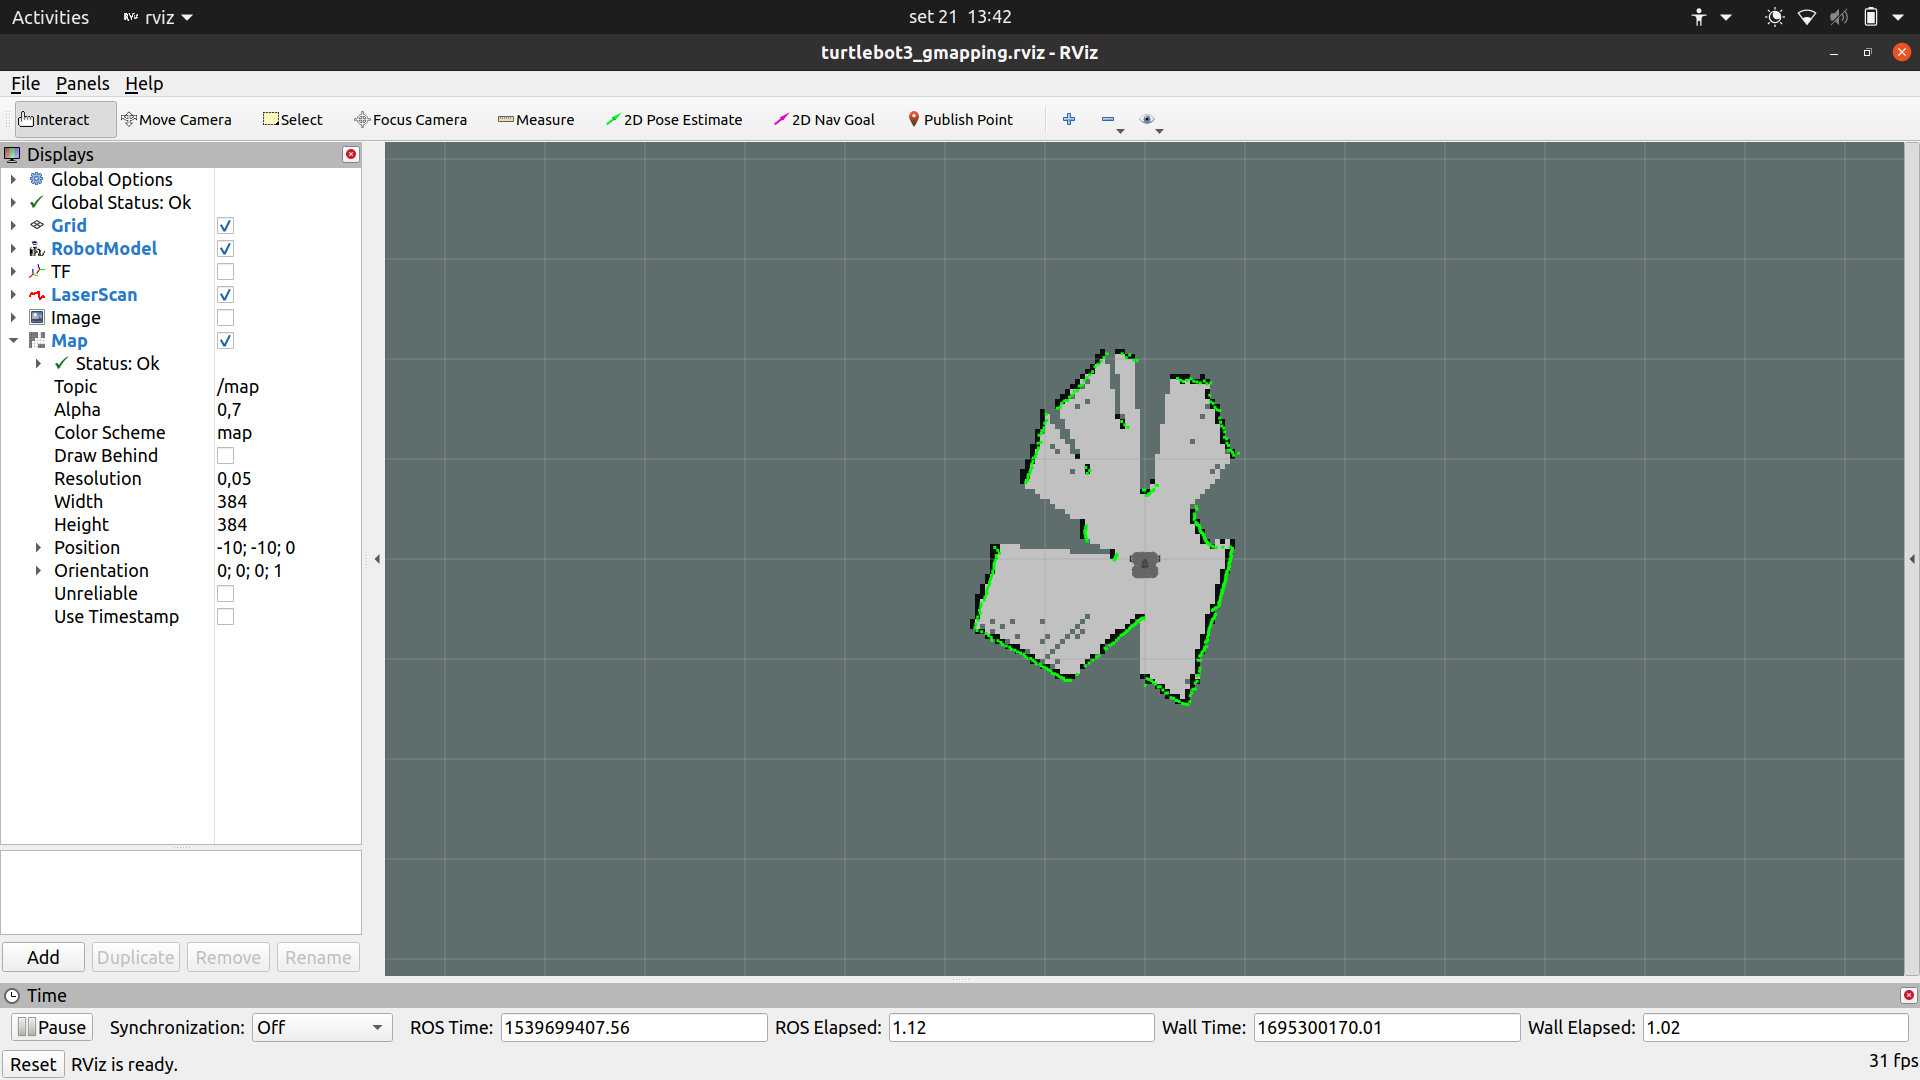
\includegraphics[width=1.0\textwidth]{./Images/dataset_gmapping_initial_map}
\caption{Dataset provided map (still mapping)}
\label{fig:flowchart}
\end{figure}


\begin{figure}[h]
\centering
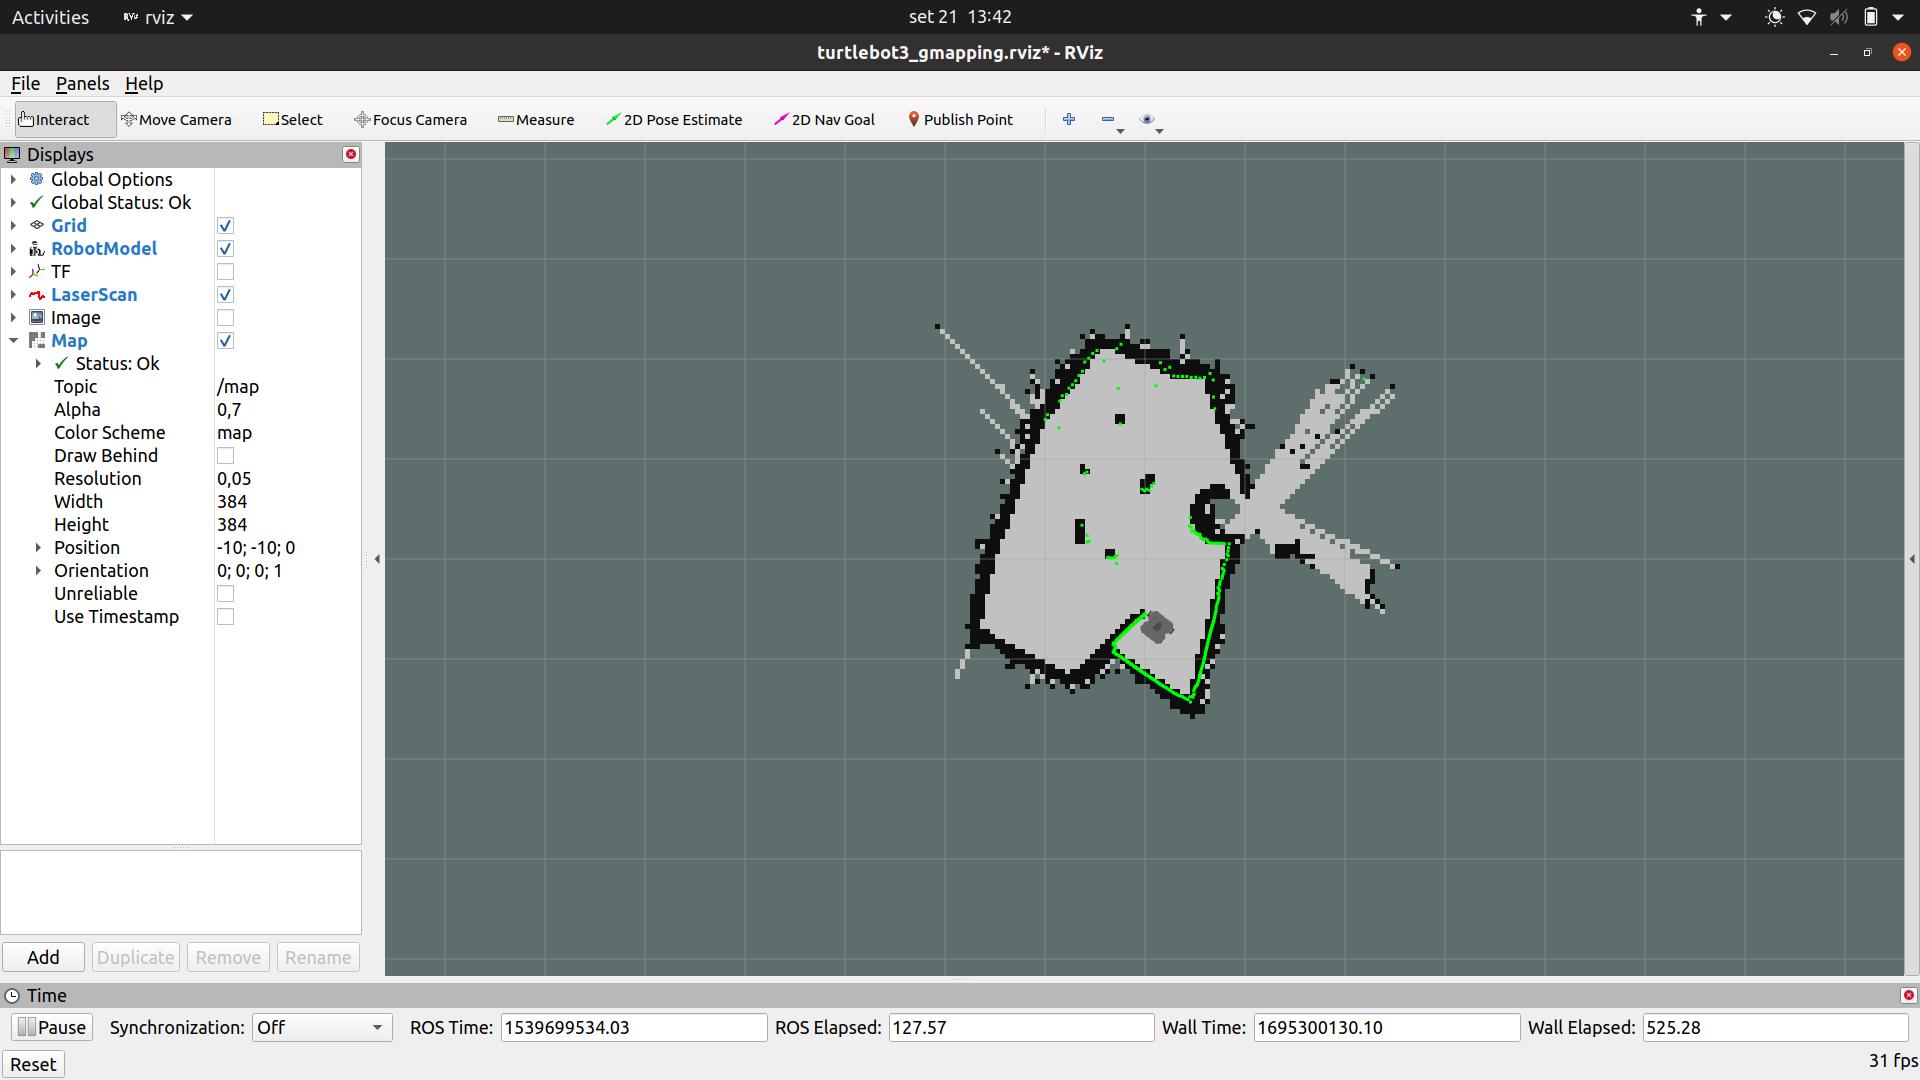
\includegraphics[width=1.0\textwidth]{./Images/dataset_gmapping_final_map}
\caption{Dataset provided map (fully mapped)}
\label{fig:flowchart}
\end{figure}

<Compare gmapping position results with ground thruth>

The same principle was then applied to map the room where we had previously recorded a rosbag. 
The results originated can be visualised in the figure bellow.

\begin{figure}[h]
\centering
\vspace{3pt}
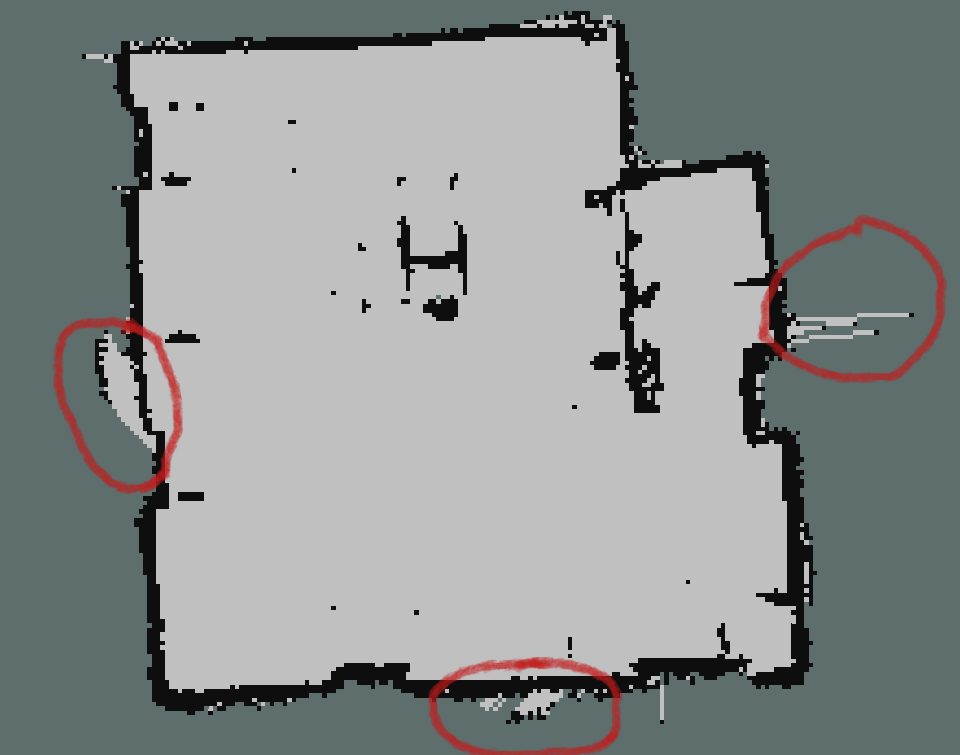
\includegraphics[scale=0.4]{./Images/lsdc4Map}
\caption{LSDC4 room map}
\label{fig:flowchart}
\end{figure}

It is possible to see some noise associated with the image. This can occur due to extent reasons such as: gmapping parameters not being well calibrated; reflections, dynamic objects or other external disturbances; sensor noise and more. The noise is represented in the figure through red circles.